\subsection{Análisis SHAP}

Después de realizar la investigación y la comparación de algoritmos, se determinó que el mejor modelo de clasificación es RandomForestClassifier, y el mejor modelo de regresión es LinearRegression, como el objetivo de la investigacion es determina la aprobacion del ramo el modelo de clasifacion RandomForestClassifier es es el mas adecuardo para realizar nuestro analisis utilizando la variable objetivo \say{aprobado} que nos permitira indentificar si aprobo o reprobo la primera evaluacion y si la guia de apoyo tiene algun impacto significativo para la aprobacion. A continuación, analizaremos los resultados de este modelo.

\subsubsection{Análisis del Mejor Modelo de Clasificación: RandomForestClassifier}


Para el análisis, se prepararon las coordenadas de análisis X/Y utilizando la columna \say{aprobado} (binaria, obtenida de \say{sol1}, donde 1 significa aprobado con una nota mayor o igual a 4) como referencia para el eje Y. Analizaremos el comportamiento de las demás columnas en relación con dicho eje X.

La selección de características y variable objetivo se presenta a continuacion:

\begin{lstlisting}[language=Python, caption=Selección de características y variable objetivo RandomForestClassifier, label=lst:seleccion_caracteristicasRFC]
    y = df["aprobado"]
    X = df[
        ['hito1', 'hito2', 'exitosos', 'fallidos', 'e0', 'e1', 'e2', 'e3', 'e4', 'e5', 'e6', 'e7', 'e8', 'e9', 'e10', 'e11', 'e12', 'e13', 'e14', 'e15', 'e16', 'e17', 'e18', 'e19', 'e20', 'e21', 'e22', 'e23', 'e24', 'e25', 'e26', 'e27', 'e28', 'e29', 'e30', 'e31', 'e32', 'e33', 'e34', 'e35', 'e36', 'e37', 'e38', 'e39', 'e40', 'e41', 'e42', 'e43', 'e44', 'e45', 'e46', 'e47', 'e48', 'e49', 'e50', 'e51', 'e52']
    ]
\end{lstlisting}

Se dividen los datos en un conjunto de entrenamiento (80\% de los datos) y un conjunto de prueba (20\% de los datos), y almacena esos conjuntos en las variables correspondientes. Esto es útil para evaluar el rendimiento del modelo en datos no vistos durante el entrenamiento.

\begin{lstlisting}[language=Python, caption=Division datos de entrenamiento, label=lst:train_test_split_RFC]
    X_train, X_test, y_train, y_test = train_test_split(X,y, test_size = 0.2,random_state= 1502)
\end{lstlisting}

Se realiza del modelo de clasificacion segun la mejor definicion de sus opciones de configuracion con el que se obtuvo el mejor resultado en la comparacion de algoritmos.

\begin{lstlisting}[language=Python, caption=Deficion de modelo RandomForestRegressor, label=lst:def_RFC]
    model = RandomForestRegressor( 
        max_depth=10, 
        min_samples_split=10, 
        min_samples_leaf=5,
        random_state= 1502,
        n_estimators=500
    )
\end{lstlisting}

Realizar Stratified K-Fold Cross-Validation en los datos de entrenamiento

\begin{lstlisting}[language=Python, caption=Realizar Stratified K-Fold Cross-Validation en los datos de entrenamiento, label=lst:skfold_train]
    # Realizar Stratified K-Fold Cross-Validation en los datos de entrenamiento
    from sklearn.model_selection import StratifiedKFold
    
    
    kfold = StratifiedKFold(n_splits=10, shuffle=True, random_state=1502)
    
    # Matrices para almacenar los resultados de validación cruzada
    cv_scores = []
    cv_predictions = []
    
    for train_index, val_index in kfold.split(X_train, y_train):
        # Dividir los datos en conjuntos de entrenamiento y validación
        X_train_fold, X_val_fold = X_train.iloc[train_index], X_train.iloc[val_index]
        y_train_fold, y_val_fold = y_train.iloc[train_index], y_train.iloc[val_index]
        
        # Entrenar el modelo en el conjunto de entrenamiento del fold actual
        model.fit(X_train_fold, y_train_fold)
    
        # Realizar predicciones en el conjunto de validación del fold actual
        y_val_pred = model.predict(X_val_fold)
    
        # Calcular el error cuadrático medio en el conjunto de validación del fold actual
        fold_score = mean_squared_error(y_val_fold, y_val_pred)
        cv_scores.append(fold_score)
    
        # Almacenar las predicciones del fold actual para su uso posterior
        cv_predictions.extend(y_val_pred)
    
        # Calcular el coeficiente de determinación en el conjunto de validación del fold actual
        r2 = r2_score(y_val_fold, y_val_pred)
        print("Fold - Error cuadrático medio:", fold_score)
        print("Fold - Coeficiente de determinación (R2):", r2)
        print()
    
    # Calcular la puntuación promedio de validación cruzada
    avg_score = np.mean(cv_scores)
    percentage_score = avg_score * 100
    print("Promedio del error cuadrático medio en validación cruzada:", avg_score)
    print("Promedio del error cuadrático medio en validación cruzada en %:", percentage_score)
\end{lstlisting}


los resultados obtenidos son los siguientes:

\begin{lstlisting}[language=Python, caption=Realizar Stratified K-Fold Cross-Validation en los datos de entrenamiento, label=lst:skfold_train]
    Fold - Error cuadrático medio: 0.22338734811732283
Fold - Coeficiente de determinación (R2): 0.0994393219751517

Fold - Error cuadrático medio: 0.21610303921931265
Fold - Coeficiente de determinación (R2): 0.13074682521909087

Fold - Error cuadrático medio: 0.23996759796803746
Fold - Coeficiente de determinación (R2): 0.029536443893225295

Fold - Error cuadrático medio: 0.20615353475177942
Fold - Coeficiente de determinación (R2): 0.1662853896389751

Fold - Error cuadrático medio: 0.21340755435714084
Fold - Coeficiente de determinación (R2): 0.13694908873044587

Fold - Error cuadrático medio: 0.212295439508615
Fold - Coeficiente de determinación (R2): 0.14144664148272745

Fold - Error cuadrático medio: 0.2277649508485301
Fold - Coeficiente de determinación (R2): 0.07888570778463855

Fold - Error cuadrático medio: 0.20885878320610823
Fold - Coeficiente de determinación (R2): 0.1553449749439464

Fold - Error cuadrático medio: 0.23418401446153864
...
Fold - Coeficiente de determinación (R2): 0.22574074537220024

Promedio del error cuadrático medio en validación cruzada: 0.21735742055519647
Promedio del error cuadrático medio en validación cruzada en %: 21.735742055519648
\end{lstlisting}

Si el RMSE es 0, significa que el modelo predice perfectamente los valores reales. Cuanto más cerca esté el MSE o RMSE de cero, mejor será el rendimiento del modelo en términos de la diferencia entre las predicciones y los valores reales.

Realizar la predicción con SHAP utilizando el conjunto de prueba

\begin{lstlisting}[language=Python, caption=Realizar Stratified K-Fold Cross-Validation en los datos de entrenamiento, label=lst:skfold_train]
    # Realizar la predicción con SHAP utilizando el conjunto de prueba (X_test)
    explainer = shap.Explainer(model)
    shap_values = explainer.shap_values(X_test)
\end{lstlisting}

A continuacion revisaremos los resultados obtenidos revisando los graficos SHAP.

Para comprender mejor los gráficos que veremos a continuación, es necesario entender lo siguiente:

\begin{itemize}
    \item El término \say{higher} se refiere a las instancias que tienen valores más altos en comparación con otras instancias, y tienen un mayor impacto en la probabilidad de ser \say{aprobado}.
    \item El término \say{lower} se refiere a las instancias con valores más bajos de la característica, que tienen un menor impacto en la probabilidad de ser \say{aprobado}.
\end{itemize}

Viendo los graficos de caracteristicas

\begin{lstlisting}[language=Python, caption=Realizar Stratified K-Fold Cross-Validation en los datos de entrenamiento, label=lst:skfold_train]
    # Mostrar Grafico de Caracteristicas
    shap.summary_plot(shap_values, X_test)
\end{lstlisting}


En la Figura \ref{fig:caract_var_shap} se muestra el gráfico de características variables SHAP gráfico.

\begin{figure}[H]
    \centering
    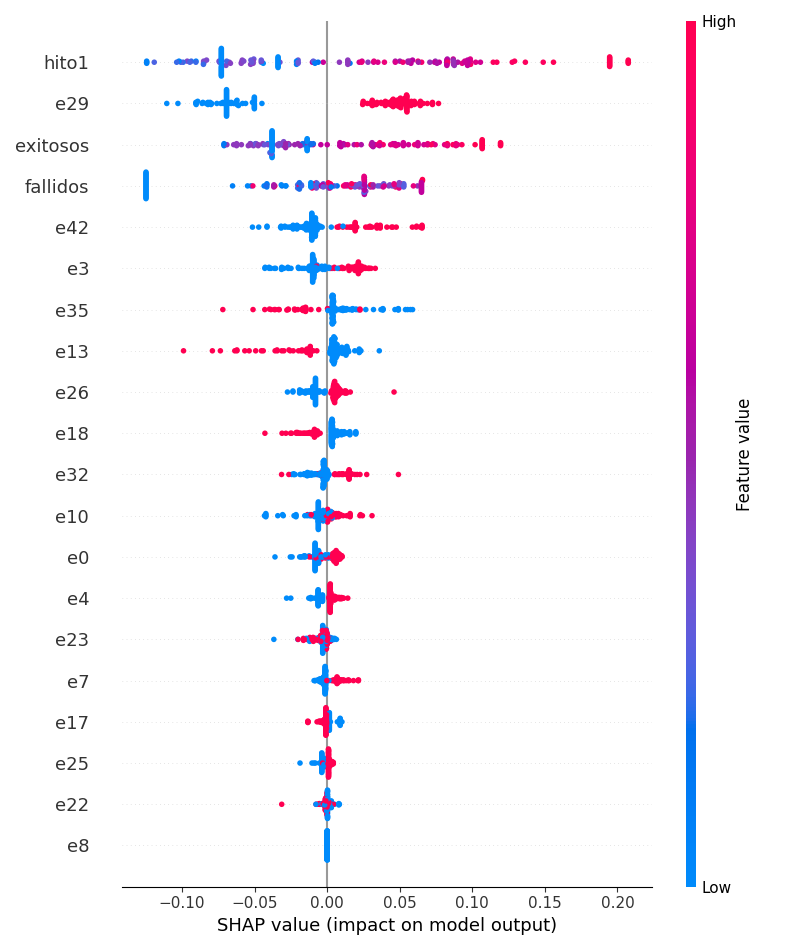
\includegraphics[width=0.5\textwidth]{img/shap_rf/shapForcePlot2.png}
    \caption{Características Variables SHAP}
    \label{fig:caract_var_shap}
\end{figure}

Al observar este podemos destacar lo siguiente:

\begin{itemize}
    \item La variable \say{hito1}  muestra un alto \say{higher} contribuyendo bastante informacion con sus picos de dispercion.
    \item La pregunta de la guía \say{e29} también es una variable de interés, siendo una de las preguntas de la guía con la mayor dispercion en sesgos \say{higher} y \say{lower}.
    \item Tanto las variables \say{exitosos} como \say{fallidos} también son variables interesantes de analizar, ya que están correlacionadas con la intención de resolver la guía.
    \item La variable \say{e42} como la variable \say{e3}, tiene un un conjunto de datos bastante marcado entre  sus colores \say{azul} y \say{rojo}.
\end{itemize}

Además, se presenta otro gráfico generado por matplotlib sobre la prediccion del modelo en la Figura \ref{fig:caract_var_shap_mat}:

\begin{figure}[H]
    \centering
    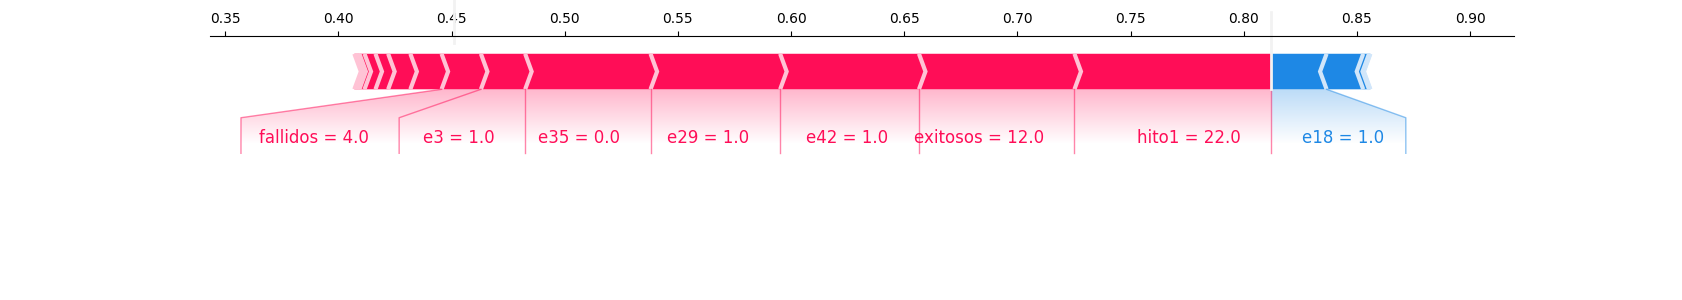
\includegraphics[width=1\textwidth]{img/shap_rf/shapForcePlot.png}
    \caption{Características Variables SHAP (Matplotlib)}
    \label{fig:caract_var_shap_mat}
\end{figure}

Al revisar este gráfico, podemos obtener más detalles sobre las características y su importancia:

\begin{itemize}
    \item La sección \say{higher} muestra los valores positivos que contribuyen a aumentar el valor de predicción. En este caso, \say{hito1} esta mas sercana a la \say{f(x)}, lo que significa que esta característica contribuye positivamente al valor de predicción en conjuntos con las variables \say{exitosos}, \say{e42}, \say{e29}, \say{e35}, \say{e3}, \say{fallidos} para \say{aprobado}.
    \item La sección \say{lower} muestra los valores negativos o fallidos que contribuyen a disminuir el valor de predicción. En este caso, la variable \say{e18}, tiene una contribución negativa al valor de prediccióno que no aporta mucho.
    \item En el gráfico, la marca \say{f(x)} representa el valor de predicción del modelo, que en este caso es 0.81.
\end{itemize}

Además de los gráficos anteriores, se presentan los gráficos de dependencia para algunas variables con referencia a \say{aprobado}:

\begin{figure}[H]

    \begin{subfigure}{0.5\textwidth}
        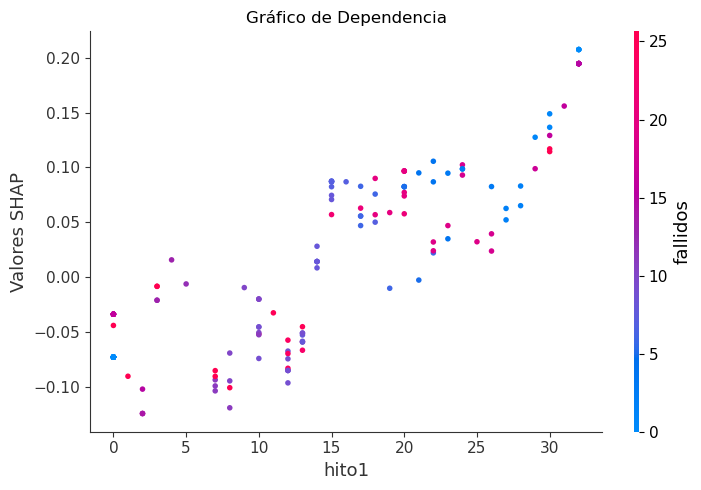
\includegraphics[width=0.9\linewidth, height=6cm]{img/shap_rf/hito1.png}
        \caption{hito1}
        \label{fig:dependencia_hito1}
    \end{subfigure}
    \begin{subfigure}{0.5\textwidth}
        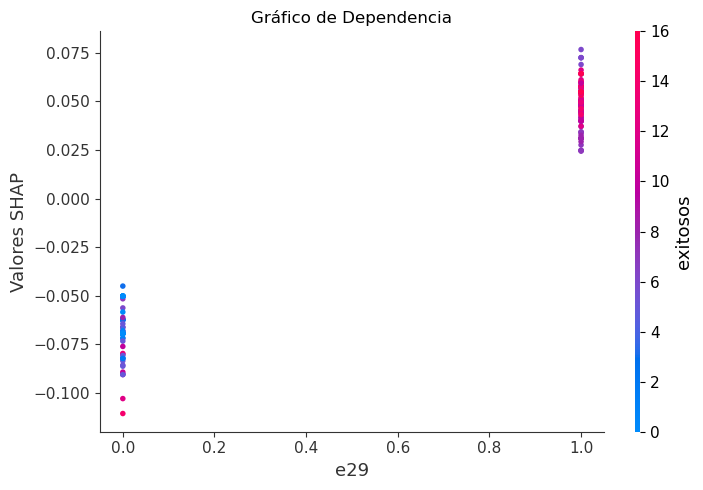
\includegraphics[width=0.9\linewidth, height=6cm]{img/shap_rf/e29.png}
        \caption{e29}
        \label{fig:dependencia_e29}
    \end{subfigure}

    \caption{Variables de dependencias hito1 - e29}
    \label{fig:image2}
\end{figure}

En la Figura \ref{fig:dependencia_hito1} se muestra el gráfico de dependencia para la variable \say{hito1} y refleja \say{fallidos} con su correlación. mientras tanto en la figura \ref{fig:dependencia_e29} se muestra el gráfico de dependencia para la variable \say{e29} con la variable \say{extisoso}.

\begin{figure}[H]

    \begin{subfigure}{0.5\textwidth}
        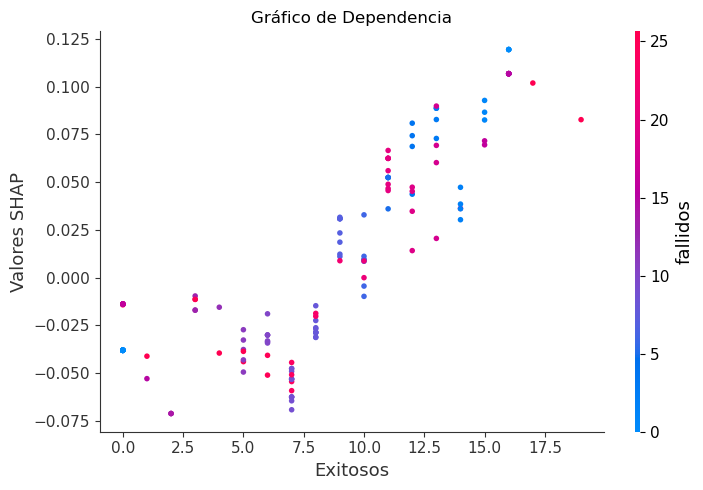
\includegraphics[width=0.9\linewidth, height=6cm]{img/shap_rf/exitosos.png}
        \caption{exitosos}
        \label{fig:dependencia_exitosos}
    \end{subfigure}
    \begin{subfigure}{0.5\textwidth}
        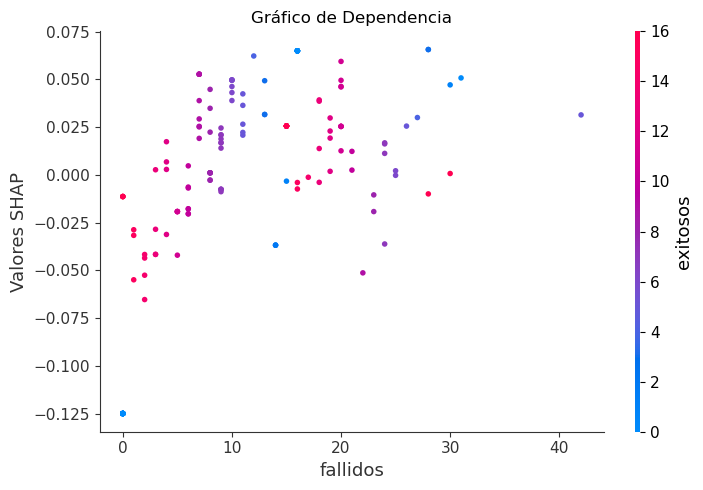
\includegraphics[width=0.9\linewidth, height=6cm]{img/shap_rf/fallidos.png}
        \caption{fallidos}
        \label{fig:dependencia_fallidos}
    \end{subfigure}

    \caption{Variable de dependencias exitosos - fallidos}
    \label{fig:image2}
\end{figure}

En la Figura \ref{fig:dependencia_exitosos} se muestra el gráfico de dependencia para la variable \say{exitosos} con su variable de dependencia \say{fallidos}, mientras tanto en la figura \ref{fig:dependencia_fallidos} se muestra el gráfico de dependencia para la variable \say{fallidos} con su dependencia \say{exitosos}.

\begin{figure}[H]

    \begin{subfigure}{0.5\textwidth}
        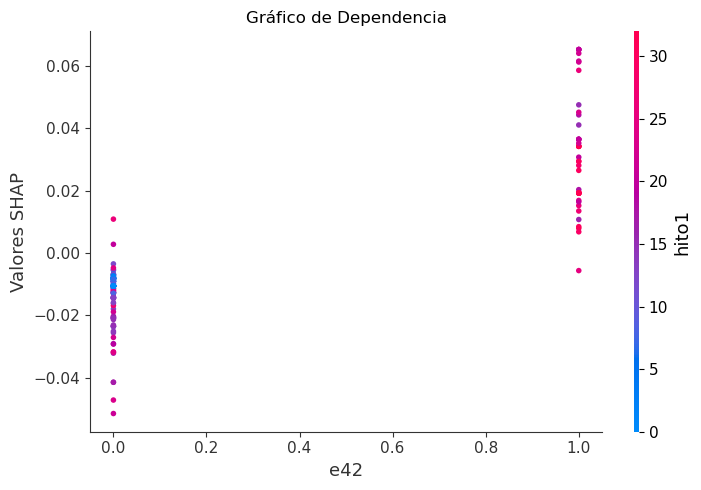
\includegraphics[width=0.9\linewidth, height=6cm]{img/shap_rf/e42.png}
        \caption{e42}
        \label{fig:dependencia_e42}
    \end{subfigure}
    \begin{subfigure}{0.5\textwidth}
        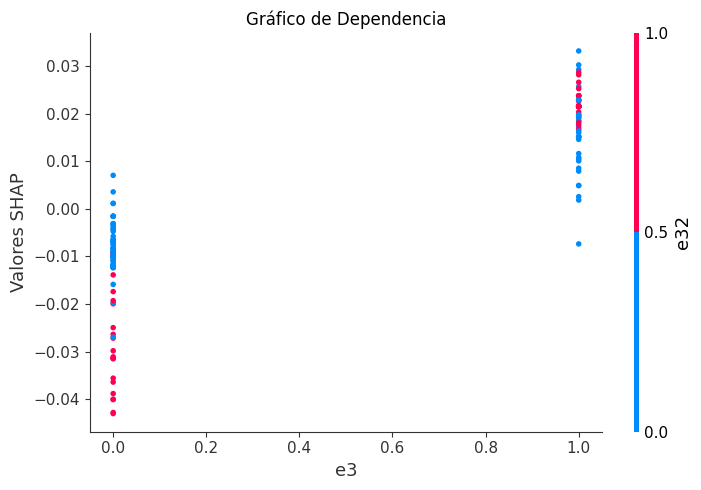
\includegraphics[width=0.9\linewidth, height=6cm]{img/shap_rf/e3.png}
        \caption{e3}
        \label{fig:dependencia_e3}
    \end{subfigure}

    \caption{Variable de dependencias e42 - e3}
    \label{fig:image2}
\end{figure}

En la Figura \ref{fig:dependencia_e42} se muestra el gráfico de dependencia para la variable \say{e42} con su dependencia \say{hito1}, mientras tanto en la figura \ref{fig:dependencia_e3} se muestra el gráfico de dependencia para la variable \say{e3} con la variable \say{e32}.

Estos gráficos de dependencia representan la relación entre los valores de las variables mencionadas y los valores de Shapley en el modelo. Proporcionan una visualización de cómo estas variables influyen en las predicciones del modelo y ayudan a comprender su importancia relativa.

En resumen, podemos entender que el modelo predictivo RandomForestClassifier tiene una función f(x) con una precisión del 81\%. Además, al observar las variables con mayor impacto en la probabilidad de ser clasificado como \textit{aprobado} (denominadas \textit{higher}), encontramos: \textit{hito1}, \textit{exitosos}, \textit{e42}, \textit{e29}, \textit{e35}, \textit{e3} y \textit{fallidos}. Por otro lado, las variables con menor impacto en la probabilidad de ser clasificado como \textit{aprobado} se encuentran en el conjunto \textit{lower}, destacando la variable \textit{e18}.

En resumen, el análisis SHAP nos ha permitido identificar las características y variables que más influyen en los modelos de clasificación. Esto nos brinda una mejor comprensión de los factores que determinan la resolucion de la guia y la nota obtenida en la prueba de conocimientos.



